%*----------- SLIDE -------------------------------------------------------------
\begin{frame}[t]{Benchmarking}
 A equipe realizou uma análise entre quatro projetos existentes que estivessem mais próximos do escopo do nosso protótipo.
    \begin{figure}
        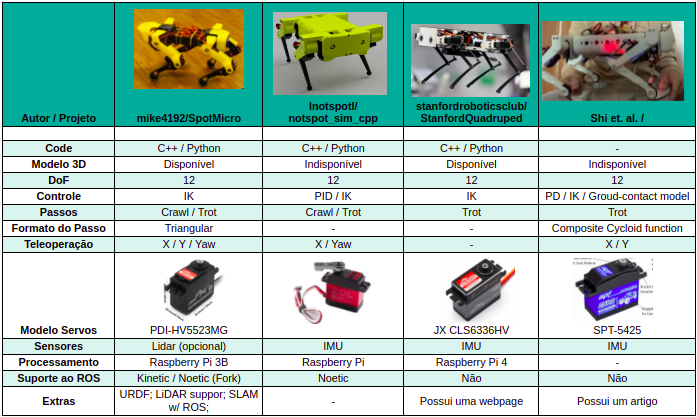
\includegraphics[ width=0.65\textwidth]{benchmarking}
        %\caption{.}
    \end{figure}
    \vspace{1cm}

%*----------- notes
    \note[item]{Notes can help you to remember important information. Turn on the notes option.}
\end{frame}
%-

%*----------- SLIDE -------------------------------------------------------------
\begin{frame}[t]{Arquitetura Geral}
    \begin{figure}
        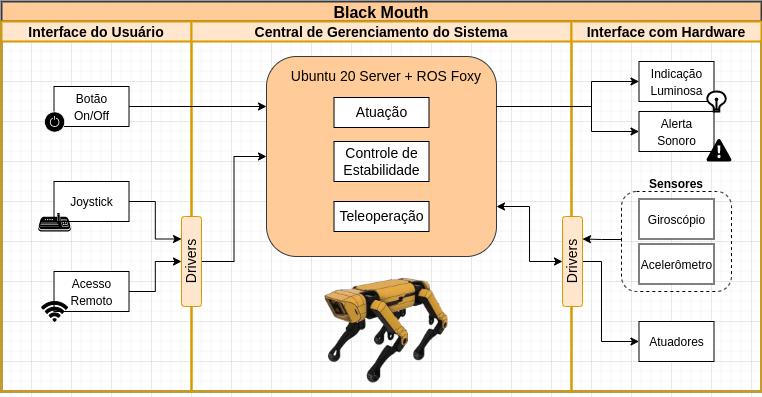
\includegraphics[width=0.85\textwidth]{arquitetura_geral.png}
        %\caption{.}
    \end{figure}
    %*----------- notes
    \note[item]{Notes can help you to remember important information. Turn on the notes option.}
\end{frame}
%-

%*----------- SLIDE -------------------------------------------------------------
\begin{frame}[t]{Project Breakdown Structure}
    \vspace{0.5cm}
    \begin{figure}
        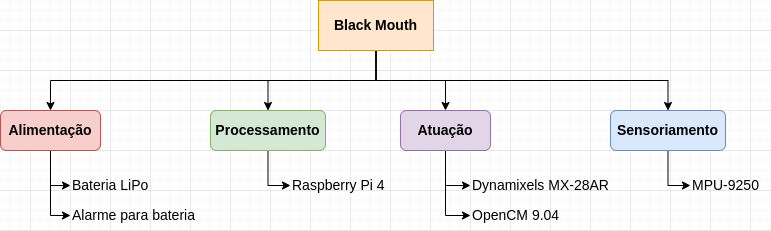
\includegraphics[width=1.0\textwidth]{PBS.png}
        %\caption{.}
    \end{figure}
    %*----------- notes
    \note[item]{Notes can help you to remember important information. Turn on the notes option.}
\end{frame}
%-

%*----------- SLIDE -------------------------------------------------------------
\begin{frame}[t]{Especificação de Funcionalidades}
    \begin{figure}
        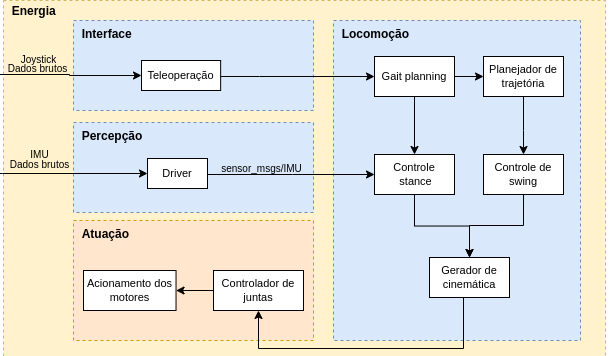
\includegraphics[width=0.78\textwidth]{funcionalidades.png}
        %\caption{.}
    \end{figure}
    %*----------- notes
    \note[item]{Notes can help you to remember important information. Turn on the notes option.}
\end{frame}
%-

%*----------- SLIDE -------------------------------------------------------------
\begin{frame}[t]{Próximas Etapas}
    \begin{columns}
        \begin{column}{0.25\textwidth}
            \begin{figure}
                
\includegraphics[width=1.0\textwidth]{next_steps.png}
                %\caption{.}
            \end{figure}            
        \end{column}
        \begin{column}{0.75\textwidth}
            \begin{itemize}
                \item \textbf{Fundamentação}
                \begin{itemize}
                    \item Finalizar escrita da Introdução
                    \item Finalizar escrita da Metodologia
                    \item Finalizar escrita da Fundamentação Teórica
                    \item Definir Design e Método de Controle     
                \end{itemize}
                \item \textbf{Desenvolvimento}
                \begin{itemize}
                    \item Elaborar CAD mecânico
                    \item Realizar projeto Elétrico-Eletrônico
                \end{itemize}
            \end{itemize}            
        \end{column}
    \end{columns}

    %*----------- notes
    \note[item]{Notes can help you to remember important information. Turn on the notes option.}
\end{frame}
%-
